\documentclass[9pt,landscape]{memoir}
\usepackage[landscape]{geometry}
\usepackage{amssymb,amsmath,verbatim,graphicx,microtype,upquote,units,booktabs,siunitx,setspace,graphicx,enumitem,siunitx,ifthen,calc,multicol,listings,xcolor}
\usepackage[absolute]{textpos}

\ifthenelse{\lengthtest { \paperwidth = 11in}}
    { \geometry{top=.1in,left=.2in,right=.2in,bottom=.1in} }
    {\ifthenelse{ \lengthtest{ \paperwidth = 297mm}}
        {\geometry{top=1cm,left=1cm,right=1cm,bottom=1cm} }
        {\geometry{top=1cm,left=1cm,right=1cm,bottom=1cm} }
    }

\setlist[description]{
 font={\bfseries\sffamily\color{red}}
}

\usepackage[colorlinks = true,
            linkcolor = red,
            urlcolor  = red,
            citecolor = red,
            anchorcolor = red]{hyperref}

\lstdefinestyle{cC++}{
    language=C++,
    basicstyle=\tiny\ttfamily,
    keywordstyle=\color{blue}\ttfamily,
    stringstyle=\color{red}\ttfamily,
    commentstyle=\color{gray}\ttfamily,
    morecomment=[l][\color{magenta}]{\#},
    showstringspaces=false,
    keepspaces=true,
    tabsize=4,
    breaklines=true,
    morekeywords={string}
}

% Answers In Read
\newcommand{\answer}[1]{\textcolor{red}{#1}}

% Turn off header and footer
\pagestyle{empty}
\renewcommand{\familydefault}{\sfdefault}

% Change lists to take less space
\setlist[itemize]{leftmargin=0pt, noitemsep, before={\vspace*{-\baselineskip}}, after={\vspace*{-\baselineskip}}}
\setlist[enumerate]{leftmargin=0pt, noitemsep, before={\vspace*{-\baselineskip}}, after={\vspace*{-\baselineskip}}}

% Define BibTeX command
\def\BibTeX{{\rm B\kern-.05em{\sc i\kern-.025em b}\kern-.08em
    T\kern-.1667em\lower.7ex\hbox{E}\kern-.125emX}}

\setlength{\parindent}{0pt}
\setlength{\parskip}{0pt plus 0.5ex}

% Change Listings Spacing
\usepackage{etoolbox}
\makeatletter
\preto{\@lstlisting}{\topsep=4pt \partopsep=2pt }
\makeatother
% -----------------------------------------------------------------------

\begin{document}

\raggedright
\footnotesize
\begin{multicols}{6}

% multicol parameters
% These lengths are set only within the two main columns
%\setlength{\columnseprule}{0.25pt}
\setlength{\premulticols}{1pt}
\setlength{\postmulticols}{1pt}
\setlength{\multicolsep}{1pt}
\setlength{\columnsep}{2pt}
\tiny

\begin{itemize}
    \item A forked process may share a Run-Time Stack with its parent. \answer{False.}
    \item A forked process may share code space with its parent. \answer{True.}
    \item A forked process shares its parent's data space at all times. \answer{False.}
    \item A thread may share a File Descriptor Table with its parent. \answer{True.}
    \item A thread may share a program counter with its parent. \answer{False.}
    \item A thread may share code space with its parent. \answer{True.}
    \item A thread may share data space with its parent. \answer{True.}
    \item An acceptable solution for implementing mutual exclusion is to let the users disable interrupts before entering a critical section and enable them after leaving the critical section. \answer{False.}
    \item Assume that you have globally defined. Show the correct way to do the the following.
\end{itemize}
\begin{lstlisting}[style=cC++,aboveskip=1pt,belowskip=1pt]
    struct Shared {
    char Name[10];
    int Value; } S1, S2;

    thread_t tid;
    void * RtnValue;
    void * FooBar(void * arg);
\end{lstlisting}

\begin{enumerate}
    \item Store "THREAD 1" in S1's Name field:  \verb$strcpy( S1.Name, "THREAD 1" );$
    \item Pass S1 in the following call:  \verb$pthread_create(&tid,NULL,FooBar, void *S1);$
    \item From within the function FooBar, print the Name that was passed inside the struct:  \texttt{printf("The Name Received = \%s\textbackslash n", ((struct Shared*)arg)->Name);}
    \item store 2 times the thread id into the Value field of arg:  \verb$((struct Shared*)arg)->Value = 2 * pthread_self();$
    \item return the struct via a thr\_exit: \verb$pthread_exit( arg );$
    \item Have main retrieve the returned value:  Use the variable RtnValue since you don't know which thread has exit-ed. Even though \verb$pthread_join()$ can be used to wait for a specific thread; there is no way to wait for "any" thread by using the Pthreads library in Linux.
    \item Have main print which thread exit-ed and the integer returned: \answer{Same.}
\end{enumerate}
\hfill
\begin{itemize}
    \item Can you build a system where mutual exclusion condition is eliminated?  \answer{No. It is a resource constraint and most resources (if not all) require it.}
    \item Can you suggest a strategy that can achieve the desired result in the previous question, i.e. no circular wait can occur in the system \answer{Assign a number to each resource and require that, at any moment, a process can only request a resource whose number is higher than that of any resource it is currently holding.}
    \item Context switch means a process switching from a ``blocked state'' to ``ready state''.  \answer{False}
    \item Create a variable named bar which stores the output of the 'users' command. \verb|bar=$(users)|
    \item Determine the output for these commands: variable="Dennis" echo ``\$variable''? \verb$Dennis$
    \item Determine the output for these commands: variable="Dennis" echo ``\$variable''? \verb|$variable|
    \item Different threads within a process may specify different dispositions for a specific interrupt \answer{True}
    \item Even if mutual exclusion is not enforced on a critical section, results of multiple execution is deterministic (i.e. it produces the same results each time it runs). \answer{False.}.
    \item Explain under what circumstances a spinlock might be less efficient than the alternative.  \answer{In uniprocessor systems, processes can use CPU one at a time.  If a process is "busy waiting" for a long time, then a spinlock might be less efficient.}
    \item Explain under what circumstances a spinlock might be more efficient than the alternative.  \answer{1. If you have more processor power than you need (e.g. in multiprocessor systems). Spinlock do not require context switch when a process must wait on a lock, and therefore it is more efficient.  2. when the locks are expected to be held for a short time, a spinlock might be more efficient (saves the context switch time, therefore, preferred).}
    \item Give an example event for each transition to occur. (You need to give at least five example events). \answer{\{create process\}: user starts a new process or a program issues a \texttt{fork()} or a \texttt{pthread\_create()} call. \{cpu available\}: the process currently occupying CPU stops running and the process in front of the READY queue is scheduled to run \{time expires\}: currently running process uses up its alloted time slot for this turn (timer interrupt). \{event wait\}: the process issues an I/O read \{event completed\}: DMA controller interrupts CPU signalling the completion of an I/O read \{exit system\}: process terminates or segmentation fault.}
    \item Give an example of something that a process might do to initiate a voluntary context switch.  Relate this answer to the Process State graph. \answer{When a process initiates an I/O Read/Write or event \texttt{wait()}. In the Process State graph, the transition is from Running State to \texttt{BLOCKED(Waiting)} State.}
    \item Give an example of something that would cause a process to experience an involuntary context switch.  Relate this answer to the Process State graph.  \answer{When a process is interrupted by an exernal source such as a timer.  In the Process State graph, the transition is from Running to Ready State.}
    \item Mach OS is a microkernal. \answer{True.}
    \item Give two reasons why we should not give the users the power to disable/enable interrupts in a multiprogrammed computer system.  \answer{(i) they may (unintentionally) forget to enable them which means all (hardware \& software) interrupts will be ignored.  (ii) they may intentionally abuse this power and let their processes dominate the system resources.}
    \item Given
\end{itemize}

\begin{lstlisting}[style=cC++,aboveskip=1pt,belowskip=1pt]
    int X[10];
    some appropriate function MyFun
    pthread_t Tid;
\end{lstlisting}

\begin{enumerate}
    \item Write the call to \verb$pthread_create()$, which executes \verb$MyFun$, which accepts the \verb$array X$ as an argument. \verb$pthread_create(&Tid, NULL, MyFun, X)$
    \item How can the code segment \verb$"if( i < y ) cout << foobar(i,y);"$ be made to behave as if it were atomic? Answer the question by recoding the segment.
\end{enumerate}

\begin{lstlisting}[style=cC++,aboveskip=1pt,belowskip=1pt]
    pthread_mutex_t m=1;
    pthread_mutex_lock( &m );
    if( i < y ) cout << foobar( i, y );
    pthread_mutex_unlock( &m );
\end{lstlisting}

\begin{itemize}
    \item How does a thread acquire RAM that is NOT shared with other threads in the task? \answer{Define local variables and use them only in this thread scope.}
    \item How does a user process get privileged operations performed? \answer{The hardware allows privileged instructions to be executed only in supervisor mode. If an attempt is made to execute a privileged instruction in user mode, the hardware does not execute the instruction, but rather treats the instruction as illegal and traps to the OS and automatically switches to supervisor mode. When a user program does a system call, the switch to the supervisor mode is done automatically by the OS and the priviledged instructions that are needed by the system routine can be executed. Since the OS code is trusted, there is no harm done by giving access to privilidged instructions this way.}
    \item I've got a variable named \verb$flibble$ which contains the string \verb$tom Jerry harry$. Write a command which stores just \verb$tom$ into a new variable. \verb|new=$(echo $flibble|\verb$ | cut -f1 -d' ')$
    \item If a process uses up its allocated time slot, a timer interrupt occurs and the process is placed in a BLOCKED Queue.  \answer{False. It is placed in the READY queue.}
    \item If mutual exclusion is not enforced in accessing a critical section, a deadlock is guaranteed to occur. \answer{False.}
    \item If the shared resources are numbered $1$ through $N$ and a process can only ask for resources that are numbered higher than that of any resource that it currently holds, then deadlock can never happen. \answer{True.}
    \item If there is no mutual exclusion condition for any resource in the system, then there is no possibility for deadlock. \answer{True.}
    \item If we constrain the resource requests in such a way that no cycle can occur in the process-resource graph, then deadlock can be prevented permanently. \answer{True.}
    \item In Producer/Consumer problem access to shared buffer must be done in a critical section, but access to ``in'' and ``out'' pointers doesn't need to be done inside a critical section.  \answer{False. ``in'' and ``out'' are shared variables. They need to be accessed inside a critical section.}
    \item In Readers/Writers problem, it is possible to write code which is functionally correct but may lead to the starvation of writers. However, it is impossible to write the code such that readers may starve instead of writers. \answer{False. It is possible to write such code.}
    \item In a uniprocessor environment, threads waiting for a lock always sleep rather than spin. Why is this true (and reasonable)? \answer{In a uniprocessor system, only one thread can run at a time. If a thread is spinning for a lock, it is doing nothing but wasting CPU cycles while waiting for the lock to become available. Instead, it is better that they sleep (in the blocked queue) while waiting so that others can use the CPU.  When the lock becomes available, OS will wake them up.}
    \item In dining philosophers problem, which senario may lead to a deadlock situation?  \answer{If the simulation code is written in such a way that each philosopher first acquires the right fork and then attempts to acquire the left fork, a deadlock may occur. Because it is possible that philosophers may enter a circular wait situation in which each one holds the fork on the right and tries to get the fork on the left (which will never happen).}
    \item In dining philosophers problem, why examining and acquiring a fork is done inside a critical section? Explain by giving an example what may go wrong if critical section is not used.  \answer{Each fork is shared by two neighboring philosophers. If it is not handled inside a critical section, both philosophers may think that they acquired the same fork and start eating using the same fork. This situation leads to an incorrect simulation.}
    \item In the specification of \verb$pthread_join()$ in Linux, there is no way to wait for "any" thread (i.e. the call should specify a particular \verb$thread_id$ to join) \answer{True.}
    Q. In the ``zombie'' state, the process no longer exists but it leaves a record for its parent process to collect. \answer{True.}
    \item LINUX is designed as a monolithic kernel. \answer{True. But, with a new twist for expanding OS functionality: LINUX supports dynamically installable modules. A module can be compiled and installed on a running version of the kernel. This is accomplished by providing system calls to install/remove modules.}
    \item Many modern O.S.s use a microkernel design.  What does that mean? \answer{Microkernel is a small privileged OS core that provides process scheduling, memory management, and communication services and relies on other processes to perform some of the functions traditionally associated with the operating system kernel. It removes all nonessential components from the kernel, and implements them as system and user-level programs. The result is a smaller kernel. Amoeba, Chorus, Mach, and Windows/NT use microkernel design approach.}
    \item Multiprogramming (having more programs in RAM simultaneously) decreases total CPU efficiency (in comparison to Uniprogramming or Batch processing). \answer{FALSE. It increases CPU efficiency (see question above)}
    \item Name at least two important differences between a POSIX thread created through a \verb$pthread_create()$ call and a child process created through a \verb$fork()$ call.  \answer{1) Threads share data space and file descriptors with the other threads and the parent process while forked process doesn't 2) a forked process has a seperate and unique PID and hence a process control block (PCB) while the threads created by a process uses their parent's PCB. 3) it takes less time to create a new thread, less time to switch between two threads within the same process, less time to terminate a thread 4) Thread Library provides more control over the execution of concurrent threads through system calls such as \texttt{pthread\_yield()}, \texttt{pthread\_suspend()}, \texttt{pthread\_kill()}, and \texttt{pthread\_continue()}}
    \item One of the solutions proposed for handling the mutual exclusion problem relies on the knowledge of relative speeds of processes/processors. \answer{False. No solution should rely on such assumptions}
    \item The word 'mutex' is short for \answer{mutual exclusion}.
    \item UNIX kernel is designed as a microkernel \answer{False. UNIX is a monolithic kernel, meaning that the process, memory, device, and file managers are all implemented in a single software module.}
    \item Unlike time sharing systems, the principal objective of batch processing systems is to minimize response time. \answer{False. Principal objective for time sharing is to minimize response time. Whereas, the principal objective for batch processing is to maximize processor use.}
    \item What are the 3 possible dispositions that a process may specify with respect to a signal (interrupt)? \answer{1) ignore signal; 2) run the default signal handler provided by the OS; 3) catch the signal and run the user's signal handler.}
    \item What are the important differences between a unix \verb$fork()$ and \verb$pthread_create()$? \answer{\texttt{fork()}: child process has the separate data space with parent process, but they have the same code space. \texttt{pthread\_create()}: threads share data space, code space, and os resources, but they have the unique thread ID, register state, stack and priority, PC counter.}
    \item What are the main goals today in the design of operating systems? \answer{Convenience for user, efficient utilization of the computer resources (CPU, memory, I/O devices), and expandibility.}
    \item What are the necessary conditions for a deadlock to exist. \answer{a) mutual exclusion; b) hold and wait; c) no preemption d) circular wait.}
    \item What does \verb$#!$ signify in a shell script? \answer{It's a special notation which tells the shell, "After this mark, read the name of the script interpreter i want to use."}
    \item What does it mean to say "\verb$rand()$ call is not MT-safe"? \answer{MT-Safe : MultiThread-Safe This means that the behavior of the function \texttt{rand()} is not stable when two threads try to use it at the same time. To get around this problem, we use MT-safe interfaces (such as \texttt{rand\_r()}). However, \texttt{rand\_r()} doesn't exist on some multithreaded operating systems (e.g. LINUX), therefore, you need to execute such calls inside a Critical Section to make sure that only one thread can call the function at any one time.}
\end{itemize}

\begin{lstlisting}[style=cC++,aboveskip=1pt,belowskip=1pt]
    pthead_mutex_t rand_mutex;
    pthread_mutex_lock( &rand_mutex );
    int a = rand() % 5;
    pthread_mutex_unlock( &rand_mutex );
\end{lstlisting}

\begin{itemize}
    \item What does it mean to say that "\verb$pthread_mutex_lock(...)$ is a blocking call"?  \answer{If the mutex lock requested by this call is held by another process, the called will be blocked until the lock is released by the current owner (via executing a \texttt{pthread\_mutex\_unlock()} call)}
    \item What does it mean to say that a library or a module is MT-Safe? \answer{MT-Safe: MultiThread-Safe which means that the behavior of the function is stable when two threads try to use it at the same time. In other words, a library/module protects its global and static data with locks and can provide a reasonable amount of concurrency.}
    \item  What does the command \verb$du$ do? \answer{figures out disk usage (size of a directory)}
    \item What function is used from within a process to send a signal to a process? \verb$kill()$
    \item What information is saved and restored during a context switch? \answer{Context switch requires saving the state of the old process and loading the saved state for the new process. Process state minimally includes current contents of registers, program counter, stack pointer, file descriptors, etc.}
    \item What is a context switch? \answer{Switching the CPU to another process.}
    \item What is a critical section i.e. what makes a section ``critical''? \answer{In an asynchronous procedure of a computer program, a part that can not be executed simultaneously with an associated critical section of another asynchronous procedure. In general, a code segment in which shared variables, shared file descriptors (shared resources) are accessed is considered a critical section.}
    \item What is a spinlock? \answer{When a process is in its critical section, any other process that tries to enter the same CS must loop continuously in the entry code of the CS until the first one gets out. The spinlock is the most common technique used for protecting a CS in Linux. It is easy to implement but has the disadvantage that locked-out threads continue to execute in a busy-waiting mode. Thus spinlocks are most effective in situations where the wait-time is expected to be very short.}
\end{itemize}

\begin{lstlisting}[style=cC++,aboveskip=1pt,belowskip=1pt]
    spin_lock(&lock) /* Critical Section */ spin_unlock(&lock)
\end{lstlisting}

\begin{itemize}
    \item What is an alternative to spinlocking?  \answer{Put the process in a wait queue, so it doesn't waste CPU cycles and allow it to sleep until the block is released.}
    \item What is an atomic operation? \answer{An operation that can not have it's execution suspended until it is fully completed. Generally, it is a single operation that can not be interrupted or divided into smaller operations.}
    \item What is dual mode operation? \answer{User mode vs. supervisor mode.}
    \item What is the difference between \verb$pthread_mutex_lock$ and \verb$pthread_mutex_trylock$? \answer{\texttt{pthread\_mutex\_lock} is a blocking call. If we try to lock a mutex that is already locked by some other thread, \texttt{pthread\_mutex\_lock} blocks until the mutex is unlocked. But \texttt{pthread\_mutex\_trylock} is a nonblocking function that returns if the mutex is already locked.}
    \item What is the difference between starvation and deadlock?  \answer{STARVATION: A condition in which a process is indefinitely delayed because other processes are always given preference. DEADLOCK: An impasse that occurs when multiple processes are waiting for the availability of a resource that will not become available because it is being held by another process that is in a similar state.}
    \item What is the effect of executing \verb$pthread_yield()$?  \answer{\texttt{pthread\_yield()}: stop executing the caller thread and yield the CPU to another thread}
    \item What is the required function prototype for the function \verb|MyFun()|? \verb|void* MyFun( void* X )|
    \item What was the original purpose/goal in the design of operating systems? \answer{To increase the efficiency of hardware.}
    \item What would you expect to see (what instructions) surrounding the `critical section' code?
\end{itemize}

\begin{lstlisting}[style=cC++,aboveskip=1pt,belowskip=1pt]
    pthread_mutex_t mp;
    pthread_mutex_lock( &mp );
    // CRITICAL SECTION
    pthread_mutex_unlock( &mp );
\end{lstlisting}



\begin{itemize}
    \item When a process resumes execution after returning from a \verb$fork()$, how can it tell if it is the original process or the new one? \answer{By the process ID which is returned by the \texttt{fork()} call. If it is equal to 0, it is the new one (child process); if it is a non-zero positive value, it is the original process.}
    \item Which of the following strategies are used for deadlock prevention (circle all that apply)?  A. Processes request all of the resources they need at once.  They either get it all or get nothing and wait until they are all available.  B. If a process needs to acquire a new resource, it must first release all resources it holds, then reacquire all it needs C. Remove the mutual exclusion condition on all of the resources D. Do not let any process hold more than 2 resources at any time.  E. Resources are numbered sequentially in a total order. A process X can only ask for Rj if Rj $>$ Ri  $\forall$Ri that X is currently holding.  \answer{A, B, E}.
    \item Which of the following would not necessarily cause a process to be interrupted? (a) Division by zero (b) reference outside user's memory space (c) page fault (d) accessing cache memory (e) end of time slice (f) none of the above \answer{d}.
    \item While DMA (Direct Memory Access) is taking place, processor is free to do other things. The processor is only involved at the beginning and end of the DMA transfer.  \answer{True.}
    \item Who are the 2 individuals generally credited with the invention of C/Unix?  \answer{Ken Thompson and Dennis Ritchie.}
    \item Why are context switches considered undesirable (to be minimized) by OS designers?  \answer{Because context switches waste a considerable amount of CPU time when they save and load the state of the processes.}
    \item Why does a machine need dual mode operation? \answer{To ensure proper operation, we must protect the operating system and all the programs and their data from any malfunctioning program.  The protection is accomplished by designating some of the machine instructions that may cause harm as "privileged" instructions.  Dual mode operations can protect the OS from errant users, and the users from one another.  It also prevents the abuse of priviledged instructions (such as 'interrupt enable/disable') by the user programs.}
    \item Write a command which lists the processes that are owned by or contain the word foo in their name. \verb$ps -ef | grep foo$
    \item Write a command which reads from the keyboard and stores it in the variable kbinput \verb$read kbinput$
    \item  Write a loop which reads the file `foobar' into the variable `lineIN' one line at a time
    \verb$cat foobar | while read lineIN  (do ... done)$
    \item Write a shell statement which divide $\frac{3}{2}$ and stores the answer in \verb|$average| \verb|average=$(echo '3 / 2'| \verb$| bc)$
    \item Write a shell statement which first adds the numbers $5$ and $7$ and stores the result in \verb|$sum|. \verb|sum=$(echo '5 + 7'| \verb$| bc)$
    \item Write an if statement which compares \verb|$variable| to the integer $5$ to see if it is equal \verb|if [ $variable -eq 5 ]|
    \item Write the command which throws output and errors away while running the script foo.sh. \verb|foo.sh >& /dev/null|
    \item Write the name of the system call for obtaining the process id of a process in UNIX? \verb$getpid()$
    \item Write the name of the system call for obtaining the process id of a process' parent in UNIX?  \verb|getppid()|
    \item If I issue the command \verb$someprogram.sh textfile$ how do i access \verb$textfile$ as a variable? \verb|$1|
    \item whats wrong with this command: \verb$PATH='cellardoor'$? \verb|$PATH| is a reserved system variable
    \item In a single processor system, there is no real multitasking. CPU time is shared among running processes. When the time slice for a running process expires, a new process has to be loaded for execution. Switching from one process or thread to another is called context switch. Process context switch involves saving and restoring process state information including program counter, CPU registers and process control block which is a relatively expensive (in terms of CPU time) operation. Similarly, thread context switch involves pushing all thread CPU registers and program counter to the thread private stack and saving the stack pointer. Thread context switch compared to process context switch is relatively cheap and fast as it only involves saving and restoring CPU registers.
    \item A semaphore, $s$, is a nonnegative integer variable that can only be changed or tested by these two atomic (indivisible/uninterruptable) functions:
\end{itemize}

\begin{lstlisting}[style=cC++,aboveskip=1pt,belowskip=1pt]
P(s) : [while(s == 0) {wait}; s=s-1;]
V(s) : [s = s + 1;]
    P0() { ...
    P(mutex);
    balance += amount;
    V(mutex);
    ... }
\end{lstlisting}

\begin{lstlisting}[style=cC++,aboveskip=1pt,belowskip=1pt]
    int pthread_create(pthread_t *thread, const pthread_attr_t *attr, void *(*start_routine) (void *), void *arg);
    attr = { scope, detachstate, stackaddr, stacksize, inheritsched, schedpolicy } || NULL
\end{lstlisting}

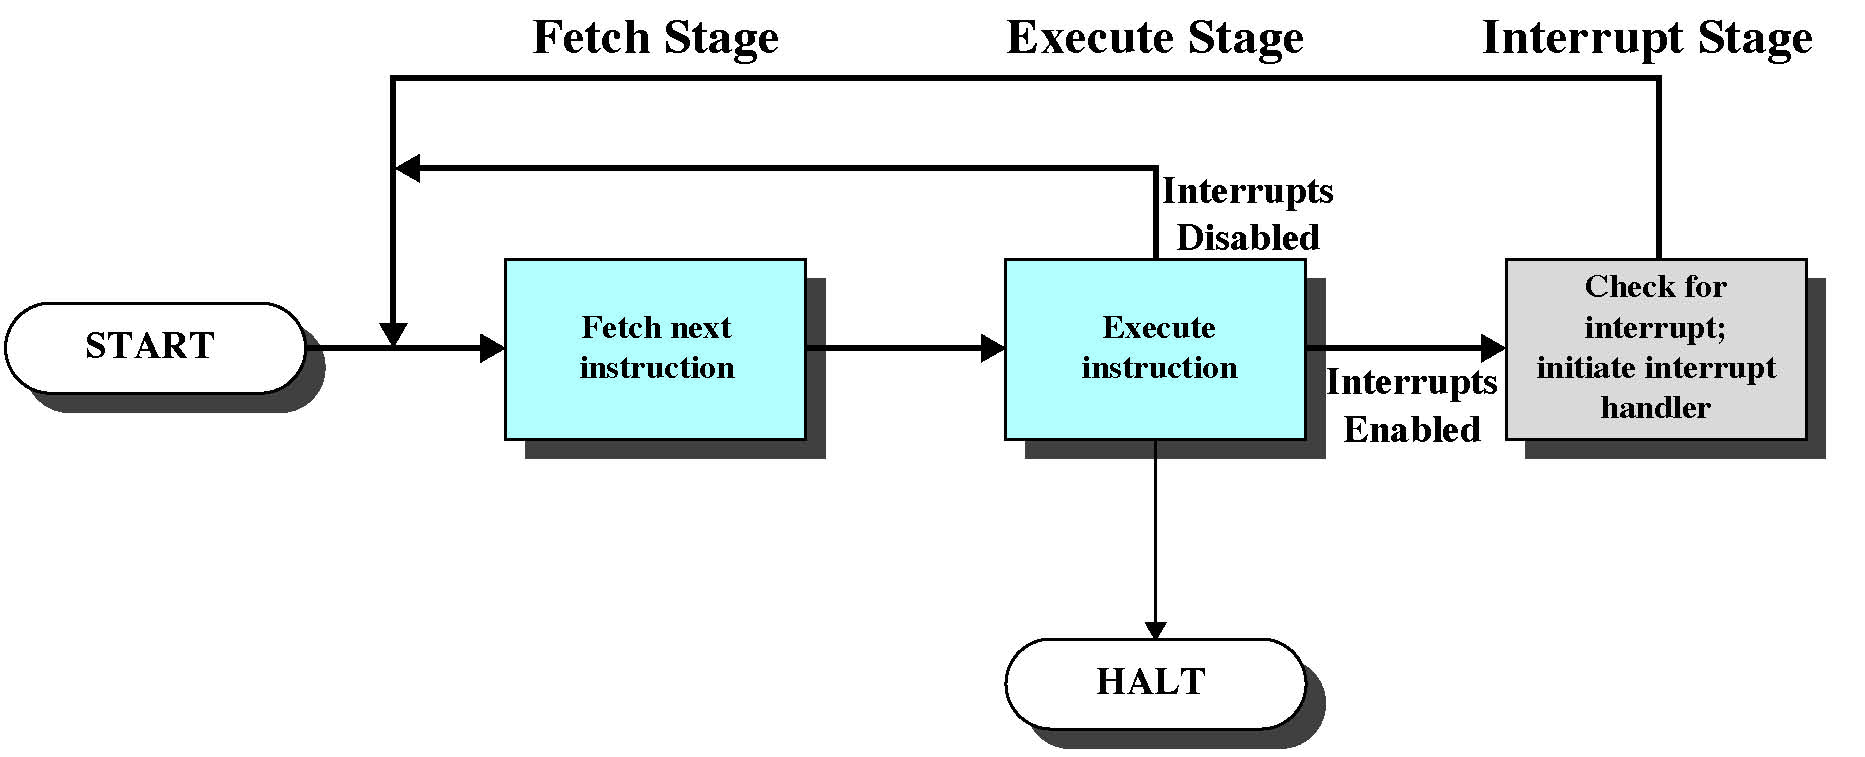
\includegraphics[width=\columnwidth]{interrupt_cycle}
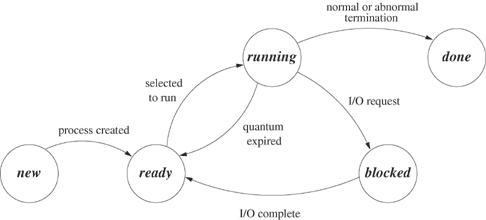
\includegraphics[width=\columnwidth]{process_state}
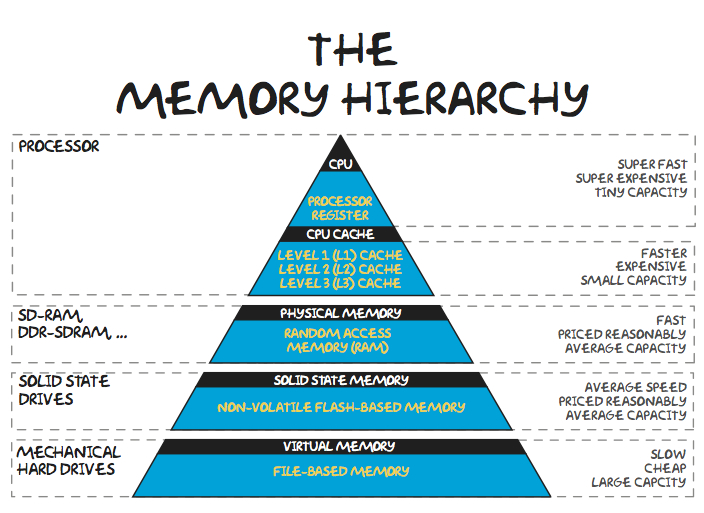
\includegraphics[width=\columnwidth]{memory-hierachy}

\miniscule
\begin{description}
    % These are the definitions likely on the test
    \item[Kernel] a portion of the operating system that includes the most heavily used portions of software. Generally— the kernel is maintained permanently in main memory. The kernel runs in a privileged mode and responds to calls from processes and interrupts from devices.
    \item[Critical Section] in an asynchronous procedure of a computer program a part that cannot be executed simultaneously with an associated critical section of another asynchronous procedure
    \item[Preemption] reclaiming a resource from a process before the process has finished using it
    \item[Concurrent] pertaining to processes or threads that take place within a common interval of time during which they may have to alternately share common resources.
    \item[Main Memory] memory that is internal to the computer system- is program addressable— and can be loaded into registers for subsequent execution of processing
    \item[Time Sharing] the concurrent use of a device by a number of users
    \item[Privileged Instruction] an instruction that can be executed only in a specific mode— usually by a supervisory program
    \item[Nonprivilaged State] an execution context that does not allow sensitive hardware instructions to be executed— such as the ‘interrupt disable’ and I/O instructions
    \item[Mutual Exclusion] a condition in which there is a set of processes— only one of which is able to access a given resource or perform a given function at any time. See critical section.
    \item[Starvation] a condition in which a process in indefinitely delayed because other processes are always given preference
    Symmetric Multiprocessing (SMP)— a form of multiprocessing that allows the operating system to execute on any available processor or on several available processors simultaneously
    \item[Shell] the portion of the operating system that interprets interactive user commands and job control language commands. It functions as an interface between the user and the operating system.
    \item[Interrupt Handler] a routine — generally part of the operating system. When an interrupt occurs — control is transferred to the corresponding interrupt handler — which takes some action in response to the condition that caused the interrupt.
    \item[Batch Processing] pertaining to the technique of executing a set of computer programs such that each is completed before the next program of the set is started
    \item[Secondary Memory] memory located outside the computer system itself— including disk and tape

    % The may or may not be on the test.
    % \item[Address Space] The range of addresses available to a computer program
    % \item[Address Translator] A functional unit that transforms virtual addresses to real addresses
    % \item[Application Programming Interface (API)] A standardized library of programming tools used by software developers to write applications that are compatible with a specific operating system or graphic user interface.
    % \item[Asynchronous Operation] An operation that occurs without a regular or predictable time relationship to a specified event; for example— the calling of an error diagnostic routine that may receive control at any time during the execution of a program
    % \item[Block] (1) a collection of contiguous records that are recorded as a unit; the units are separated by interblock gaps. (2) a group of bits that are transmitted as a unit.
    % \item[Busy waiting] the repeated execution of a loop of code while waiting for an event to occur
    % \item[Cache Memory] a memory that is smaller and faster than main memory and that is interposed between the processor and main memory. The cache acts as a buffer for recently used memory locations.
    % \item[Client] a process that requests services by sending messages to server processes
    % \item[Cluster] a group of interconnected whole computers working together as a unified computing resource that can create the illusion of being one machine. The term whole computer means a system that can run on its own apart from the cluster.
    % \item[Deadlock] (1) an impasses that occurs when multiple processes are waiting for the availability of a resource that will not become available because it is being held by another process that is in a similar wait state
    % \item[Device Driver] an operating system module (usually in the kernel) that deals directly with a device or I/O module
    % Direct Memory Access (DMA) a form of I/O in which a special module called a DMA module controls the exchange of data between main memory and an I/O device. The processor sends a request for the transfer block of data to the DMA module and is interrupted only after the entire block has been transferred.
    % \item[Disabled Interrupt] a condition usually created by the operating system during which the processor will ignore interrupt request signals of a specified class
    % \item[Disk Cache,a buffer]  usually kept in main memory that functions as a cache of disk blocks between disk memory and the rest of main memory
    % \item[Distributed Operating System] a common operating system shared by a network of computers. The distributed operating system provides support for interprocess communication process migration mutual exclusion and the prevention or detection of deadlock.
    % \item[Enabled Interrupt] a condition usually created by the operating system during which the processor will respond to interrupt request signals of a specified class
    % \item[Encryption] the conversion of plain text or data into unintelligible form by means of a reversible mathematical computation
    % \item[Execution Context] same as process state
    % \item[File] a set of related records treated as a unit
    % \item[File Allocation Table (FAT)] a table that indicates the physical location on secondary storage of the space allocated to a file. There is one file allocation table for each file.
    % \item[File Management System] a set of system software that provides services to users and applications in the use of files including file access — directory maintenance — and access control.
    % \item[First In First Out (FIFO)] a queuing technique in which the next \item to be retrieved is the \item that has been in the queue for the longest time
    % \item[Hash File] a file in which records are accessed according to the values of a key field. Hashing is used to locate a record on the basis of its key value.
    % \item[Hashing] the selection of a storage location for an \item of data by calculating the address as a function of the contents of the data. This technique complicates the storage allocation function but results in rapid random retrieval.
    % \item[Hit Ratio] in a two-level memory — the fraction of all memory accesses that are found in a the master memory (i.e. the cache)
    % \item[Interrupt] a suspension of a process — such as the execution of a computer program — caused by an even external to that process and performed in such a way that the process can be resumed
    % \item[Job] a set of computational steps packaged to run as a unit
    % \item[Job Control language (JCL)] a problem-oriented language that is designed to express statements in a job that are used to identify the job or to describe its requirements to an operating system
    % \item[Lightweight Process] a thread
    % \item[Macrokernel] a large operating system core that provides a wide range of services
    % \item[Message] a block of information that may be exchanged between processes as a means of communication
    % \item[Microkernel] a small privileged operating system core that provides process scheduling— memory management— and communication services and relies on other processes to perform some of the functions traditionally associated with the operating system kernel
    % \item[Mode Switch] a hardware operation that occurs that causes the processor to execute in a different mode (kernel or process). When the mode switches form process to kernel— the program counter— processor status word— and other registers are saved. When the mode switches from kernel to process— this information is restored.
    % \item[Monolithic Kernel] a large kernel containing virtually the complete operating system— including scheduling— file system— device drivers— and memory management. All the functional components of the kernel have access to all of its internal data structures and routines. Typically— a monolithic kernel is implemented as a single process— with all elements sharing the same address space.
    % \item[Multiprocessing] a mode of operation that provides for parallel processing by two or more processors of a multiprocessor
    % \item[Multiprocessor] a computer that has two or more processors that have common access to a main storage
    % \item[Multiprogramming] a mode of operation that provides for the interleaved execution of two or more computer programs by a single processor. The same as multitasking— using different terminology.
    % \item[Multitasking] a mode of operation that provides for the concurrent performance or interleaved execution of two or more computer tasks. The same as multiprogramming— using different terminology.
    % \item[Network Operating System] the software— supplemental to the operating system— that provides support for the use of common server systems in a network of computers
    % \item[Operating System] software that controls the execution of programs and that provides services such as resource allocation— scheduling— input/output control— and data management
    % \item[Process] a program in execution. A process is controlled and scheduled by the operating system. Same as task.
    % \item[Process Control Block] the manifestation of a process in an operating system. It is a date structure containing information about the characteristics and state of the process.
    % \item[Process Descriptor] same as process control block
    % \item[Process Image] all of the ingredients of a process— including program— data— stack— and process control block
    % \item[Process State] all of the information that the operating system needs to manage a process and that the processor needs to properly execute the process. The process state includes the contents of the various processor registers— such as the program counter and data registers; it also includes information of use to the operating system— such as the priority of the process and whether the process is waiting for the completion of a particular I/O event. Same as execution context.
    % \item[Process Switch] an operation that switches the processor from one process to another- by saving all the process control block— registers— and other information for the first and replacing them with the process information for the second
    % \item[Round Robin] a scheduling algorithm in which processes are activated in a fixed cyclic order. Those which cannot proceed because they are waiting for some event (e.g.— termination of a child process or an input/output operation) simply return control to the scheduler.
    % \item[Stack] a list that is constructed and maintained so that the next data \item to be retrieved is the most recently stored \item in the list. This method is characterized as last-in-first-out
    % \item[Synchronization] situation in which two or more processes coordinate their activities based on a condition
    % \item[Task] same as process
    % \item[Thread] an execution context that is independently scheduled but shares a single address space with other threads
    % \item[Time Slicing] a mode of operation in which two or more processes are assigned quanta of time on the same processor
\end{description}

Download source on \href{https://github.com/IllyaStarikov/cs3800}{my Github}.

\end{multicols}
\end{document}
